\documentclass[11pt,aspectratio=169,xcolor={dvipsnames},usepdftitle=false]{beamer}
\usepackage{presentation}
\usepackage{xspace}

\newcommand{\eg}{\emph{e.g.},\xspace}
\newcommand{\ie}{\emph{i.e.},\xspace}
\newcommand{\etc}{\emph{etc.}\xspace}
\newcommand{\etal}{\emph{et al.}\xspace}
\newcommand{\vs}{\emph{vs.}\xspace}
\newcommand{\wrt}{\emph{w.r.t.}\xspace}
\newcommand{\aka}{a.k.a.\xspace}
\hypersetup{pdfpagemode=FullScreen,hidelinks,pdfdisplaydoctitle=true,%
%
% Enter presentation title to populate PDF metadata:
pdftitle={Minimalist LaTeX Template for Academic Presentations}}

% Enter path to PDF file with figures:
\newcommand{\pdf}{figures.pdf}


% Enter title:
\title{Reinforcement Learning: \\model-free methods}

% Enter authors:
\author{Jiahui Fu}

% Enter location and date:
\date{2026.04.14}

\begin{document}
\frame{\titlepage}

\begin{frame}
\frametitle{Reinforcement Learning vs Imitation Learning} 
\begin{center}
    \includegraphics[width=0.8\textwidth]{imgs/RL_IL.png}
\end{center}
\end{frame}

\begin{frame}
\frametitle{Reinforcement Learning vs Imitation Learning}
RL provides action-level credit assignment via advantage signals.
\begin{itemize}
	\item \textbf{Formulation}\\
	\textbf{Behavior Cloning (IL):}
	\vspace{-1.2em}
	$$
	\nabla_\theta J_{BC} =
	\mathbb{E}_{(s,a)\sim\mathcal{D}_{expert}}
	\left[\nabla_\theta \log \pi_\theta(a|s)\right]
	=
	\mathbb{E}\left[
	\frac{1}{\pi_\theta(a|s)} \nabla_\theta \pi_\theta(a|s)
	\right]
	$$
    \vspace{-1.5em}
	\textbf{Policy Gradient (RL):}
	\vspace{-1.5em}
	$$
	\nabla_\theta J_{RL} =
	\mathbb{E}_{(s,a)\sim \pi_\theta}
	\left[A^\pi(s,a)\nabla_\theta \log \pi_\theta(a|s)\right]
	$$

    \vspace{-1.0em}
	\item \textbf{Key difference}

	\begin{itemize}
		\item BC: likelihood-based weighting
		\item RL: advantage-based weighting
	\end{itemize}

	\item \textbf{Implication}

	\begin{itemize}
		\item BC only increases expert action probability
		\item RL can \textbf{reinforce or suppress} actions via $A^\pi$
	\end{itemize}

\end{itemize}

\end{frame}

\begin{frame}
\frametitle{Reinforcement Learning vs Imitation Learning}
RL mitigates compounding error by learning under its own state distribution.
\begin{itemize}

	\item \textbf{Formulation}
        $$
        J(\pi_{BC}) \le J(\pi^*) + \sum_{t=1}^{T} O(t\epsilon) = J(\pi^*) + O(T^2 \epsilon)
        $$
        $$
        J(\pi_{RL}) \approx O(T \epsilon)
        $$
	\item \textbf{Key difference}

	\begin{itemize}
		\item BC: quadratic error growth
		\item RL: linear error growth
	\end{itemize}

	\item \textbf{Mechanism}

	\begin{itemize}
		\item BC is trained on $s \sim \mathcal{D}_{expert}$ (open-loop), execution uses $s \sim \pi_\theta$ → distribution shift
		\item RL trains on-policy → includes recovery states
	\end{itemize}

\end{itemize}

\end{frame}

\begin{frame}
\frametitle{Reinforcement Learning vs Imitation Learning}
RL can explicitly penalize worst-case outcomes during optimization.
\begin{itemize}
	\item \textbf{Formulation}

	\textbf{Expectation objective:}
	\vspace{-1.2em}
	$$
	\max_\theta \ \mathbb{E}[R]
	$$

	\textbf{Tail-risk penalized objective:}
	\vspace{-1.2em}
	$$
	\max_\theta \ \mathbb{E}[R]-\lambda\,\mathbb{E}\big[(\tau-R)_+\big]
	$$

	\item \textbf{Key difference}

	\begin{itemize}
		\item IL: imitates expert actions and cannot directly reweight rare bad outcomes
		\item RL: can assign stronger penalty to low-return (tail-risk) events
	\end{itemize}

	\item \textbf{Mechanism}

	\begin{itemize}
		\item RL objective is \textbf{modifiable} (reward / penalty shaping)
		\item Increase penalty weight for unsafe actions → safer policy
	\end{itemize}

\end{itemize}

\end{frame}

\begin{frame}
\frametitle{Reinforcement Learning vs Imitation Learning}

RL learns from richer supervision through environment feedback.

\begin{itemize}

	\item \textbf{Supervision source}

	\textbf{Imitation Learning (IL):}
	\vspace{-1.0em}
	$$
	(s, a^*)
	$$

	\textbf{Reinforcement Learning (RL):}
	\vspace{-1.0em}
	$$
	(s, a, r, s')
	$$

	\item \textbf{Key difference}

	\begin{itemize}
		\item IL only observes which action the expert takes
		\item RL additionally observes the outcome of each action
	\end{itemize}

	\item \textbf{Mechanism}

	\begin{itemize}
		\item reward provides explicit task-level evaluation
		\item next-state transition reveals the consequence of an action
	\end{itemize}

\end{itemize}

\end{frame}


\begin{frame}
\frametitle{Overview of Model-Free RL Methods}
    \textbf{Problem setting:} sequential decision making under environment feedback
	\vspace{-1.0em}
	$$
	\max_\pi \ \mathbb{E}_{\tau \sim \pi}\left[\sum_{t=0}^{T}\gamma^t r_t\right]
	$$
    \centering
    \begin{minipage}{0.48\textwidth}
    \centering
    \begin{itemize}

	\item \textbf{Key challenge:}
	actions affect not only immediate reward, but also future states

	\item \textbf{Model-free vs. model-based}

	\begin{itemize}
		\item model-based RL: learns or uses transition dynamics $p(s'|s,a)$
		\item model-free RL: learns policy / value directly from sampled interaction
	\end{itemize}

    \end{itemize}
    \end{minipage}
    \hfill
    \begin{minipage}{0.48\textwidth}
    \centering
    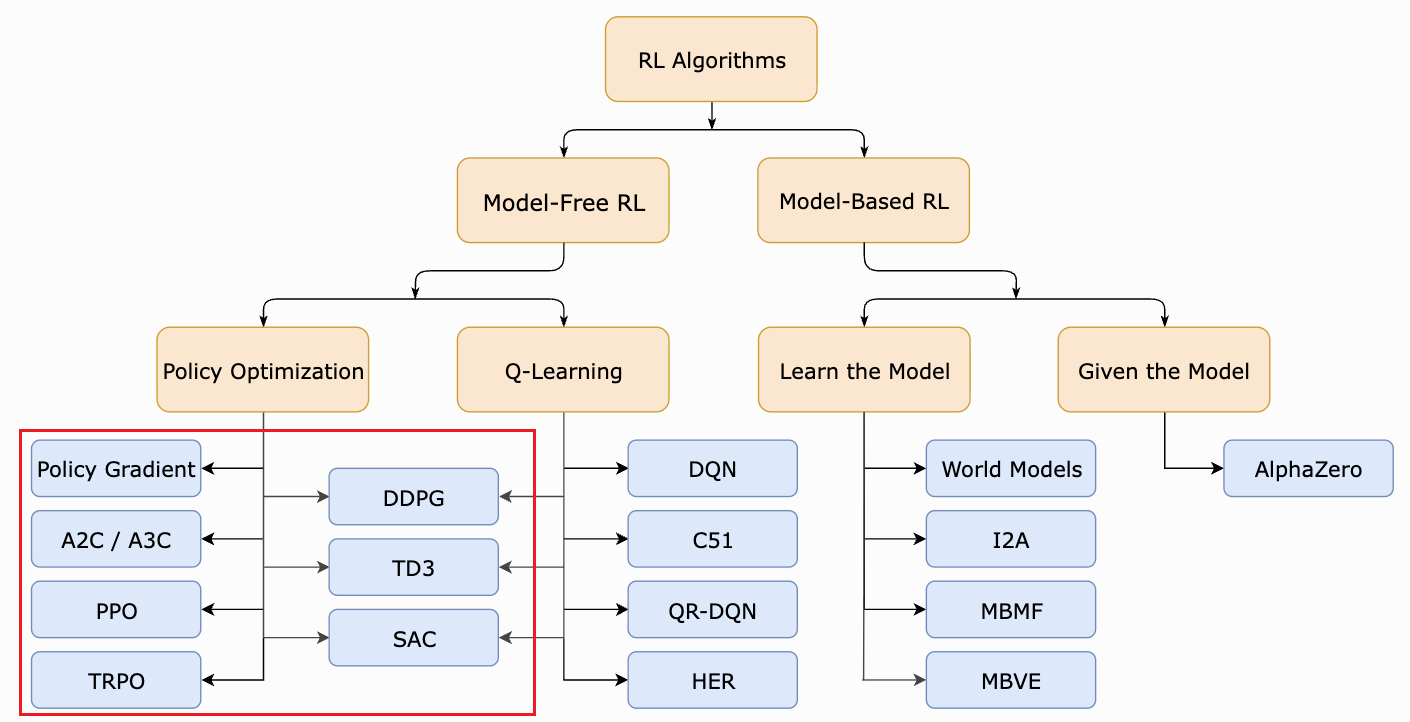
\includegraphics[width=\textwidth]{imgs/method_overview.png}
    {\small A Taxonomy of RL Algorithms}
\end{minipage}
\end{frame}


\begin{frame}
\frametitle{Overview of Model-Free RL Methods}
	\begin{minipage}{0.55\textwidth}
	\begin{itemize}
	\item Policy (Actor): $\pi_\theta(a|s)$ maps state $s$ to action $a$
	\item Environment: given $a_t$, returns reward $r_t$ and next state $s_{t+1}$
	\end{itemize}

	\vspace{0.5em}
	\textbf{Interaction and Learning}
	\begin{itemize}
	\item Rollout trajectories: $\tau = (s_0,a_0,r_0,\dots,s_T)$
	\item Compute return: $G_t = \sum_{k=t}^{T} \gamma^{k-t} r_k$
	\item Update policy to increase probability of actions with higher return
	\end{itemize}
	\end{minipage}
    \hfill
    \begin{minipage}{0.4\textwidth}
    \centering
    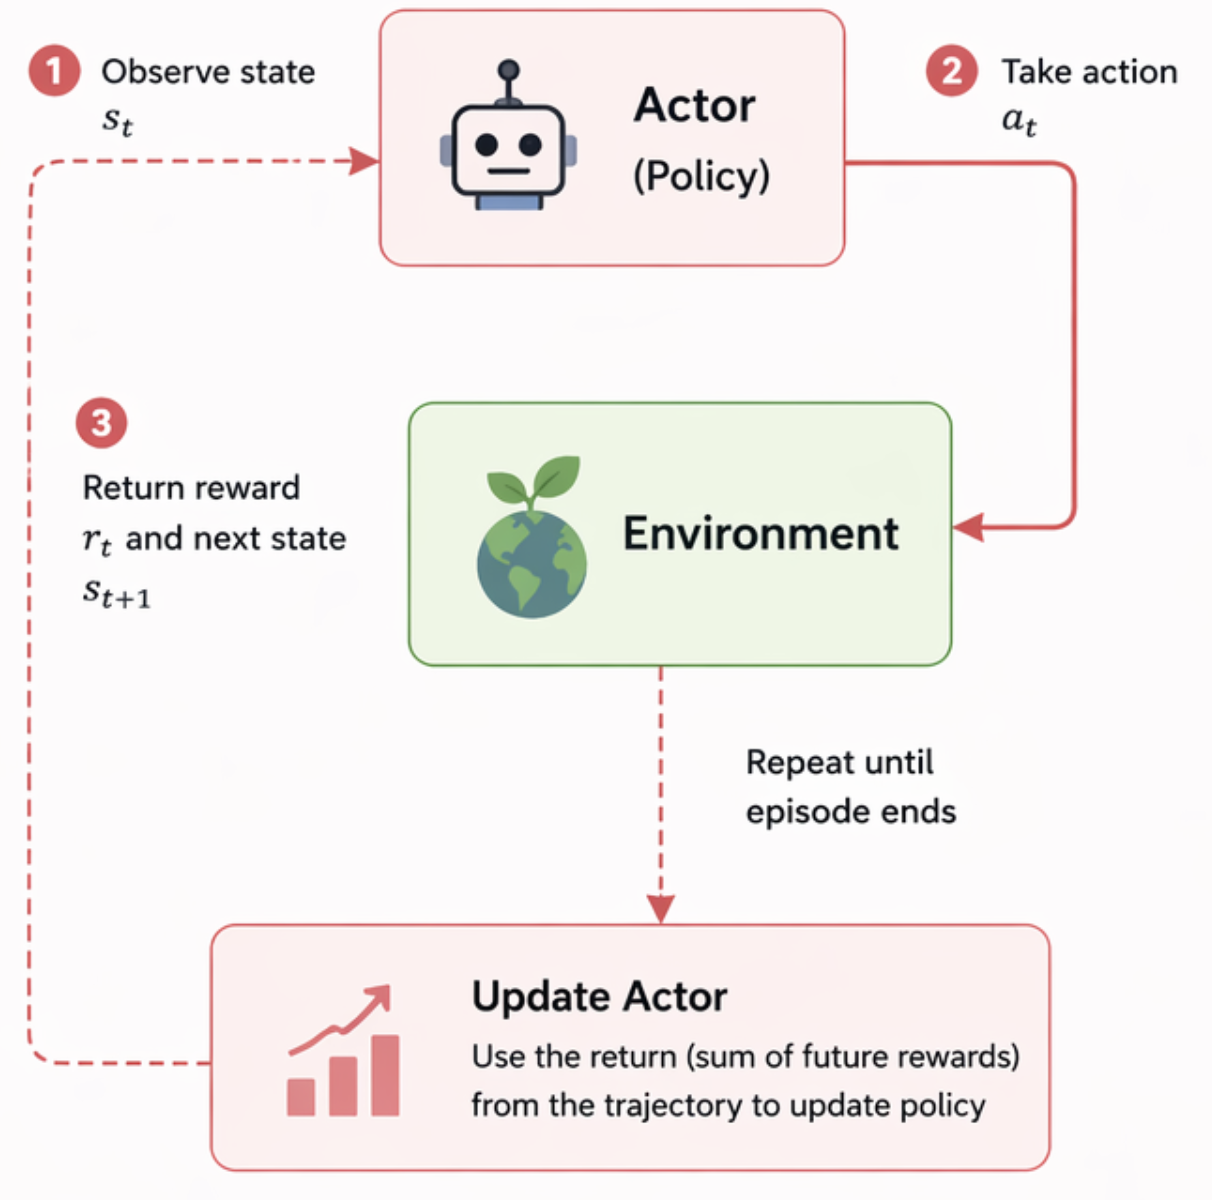
\includegraphics[width=\textwidth]{imgs/without_critic.png}
    {\small Actor-Critic Framework}
    \end{minipage}
\end{frame}


\begin{frame}
\frametitle{Overview of Model-Free RL Methods}
	\begin{minipage}{0.55\textwidth}
	\textbf{Limitation of Policy-only Methods}

	\begin{itemize}
	\item Learning signal = Monte Carlo return $G_t$
	\item High variance due to delayed and noisy rewards
	\end{itemize}

	\vspace{0.5em}

	\textbf{Introduce Critic}

	\begin{itemize}
	\item Critic learns a value function: state value $V(s)$ or action value $Q(s,a)$
	\item $V(s)$ estimates the expected future reward from state $s$, 
		and $Q(s,a)$ estimates the expected future reward after taking action $a$ in state $s$
	\item These value estimates provide a more immediate and less noisy learning signal, guiding the actor to update policy more stably
	\end{itemize}

	\end{minipage}
    \hfill
    \begin{minipage}{0.4\textwidth}
    \centering
    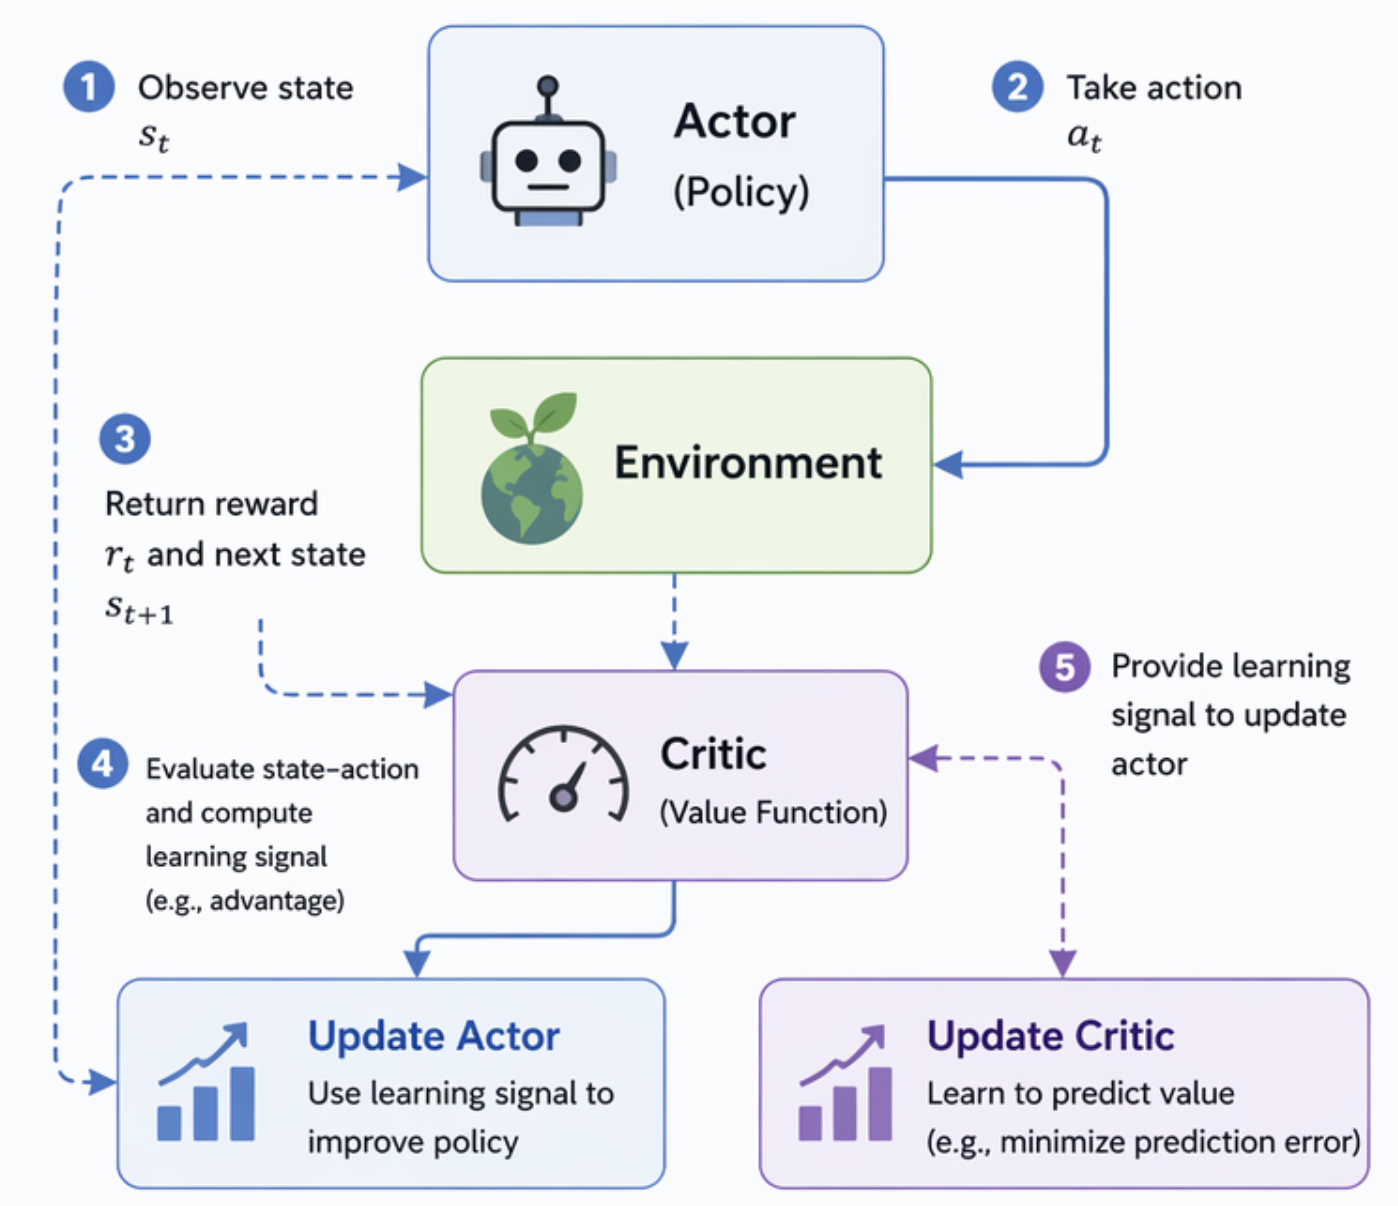
\includegraphics[width=\textwidth]{imgs/with_critic.png}
    {\small Actor-Critic Framework}
    \end{minipage}
\end{frame}


\begin{frame}
\frametitle{Deep Q-Network (DQN)}
\begin{itemize}
	\item \textbf{Motivation:} Use a neural network $Q_\theta(s,a)$ to replace Q-learning table and approximate action values in large or continuous state spaces.
	
	\item \textbf{Training target:}
	\vspace{-1.5em}
    $$
	y_t = r_t + \gamma \max_{a'} Q_{\theta}(s_{t+1}, a')
	$$
	Minimize temporal-difference error:
	\vspace{-1.0em}
    $$
	\mathcal{L}(\theta)=\mathbb{E}_{(s,a,r,s')\sim\mathcal{D}}\left[(y_t-Q_\theta(s,a))^2\right]
	$$
    \vspace{-1.5em}
	\item \textbf{Policy:}
	Given state $s$, choose action by
    \vspace{-1.0em}
	$$
	a^* = \arg\max_a Q_\theta(s,a)
	$$
    \vspace{-1.5em}
    \begin{itemize}
	\item During training, often use $\epsilon$-greedy for exploration.
	\item During evaluation, usually use greedy action selection.
    \end{itemize}
    

\end{itemize}
\end{frame}


\begin{frame}
\frametitle{DQN: Experience Replay}
\begin{itemize}
	\item \textbf{Core idea:}
	Store transitions in a fixed-capacity replay buffer $\mathcal{D}$,
	then sample random mini-batches for training.

	\item \textbf{Transition format:}
	$$
	(s_t, a_t, r_t, s_{t+1}, d_t), \quad d_t \in \{0,1\}
	$$
	where $d_t=1$ indicates episode termination.

	\item \textbf{Why it helps:}
	\begin{itemize}
		\item \textbf{Break temporal correlation:}
		Random mini-batch sampling from $\mathcal{D}$ decorrelates consecutive data.

		\item \textbf{Improve sample efficiency:}
		Stored transitions can be reused many times, reducing expensive environment interactions.

		\item \textbf{Smooth distribution shift:}
		Mixing old and new data in $\mathcal{D}$ smooths distribution and reduces oscillation.
	\end{itemize}

\end{itemize}
\end{frame}

\begin{frame}
\frametitle{DQN: Target Network}
\begin{itemize}
	\item \textbf{Core idea:}
	Maintain two Q-networks:
	$Q_\theta$ (online, updated every step) and
	$Q_{\theta^-}$ (target, updated slowly).

	\item \textbf{TD target construction:}
	\vspace{-1.0em}
    $$y = r + \gamma (1-d)\max_{a'}Q_{\theta^-}(s',a')$$
	Using $Q_{\theta^-}$ avoids chasing a rapidly moving target.

	\item \textbf{How to update $Q_{\theta^-}$:}
	\begin{itemize}
        \item \textbf{Hard update:} copy online weights every $C$ steps: $\theta^- \leftarrow \theta$.
        \item \textbf{Soft update:}: $\theta^- \leftarrow \tau\theta + (1-\tau)\theta^-$ with $\tau \ll 1$.
    \end{itemize}

	\item \textbf{Why it helps:}
	Makes labels relatively stable in short windows and reduces divergence risk.
\end{itemize}
\end{frame}


\begin{frame}
\frametitle{Deep Deterministic Policy Gradient (DDPG)}
\begin{itemize}
	\item \textbf{Motivation:}
	DQN requires solving $a^*=\arg\max_a Q(s,a)$,
	which is infeasible in continuous action spaces (\eg steering angle, throttle, brake in autonomous driving).

	\item \textbf{Training target:}
	Introduce a deterministic actor to replace $\arg\max$:
	\begin{itemize}
		\item \textbf{Actor:} $a = \mu_\phi(s)$
		\item \textbf{Critic:} $Q_\theta(s,a)$
	\end{itemize}
    Update actor and critic iteratively:

	\item \textbf{Critic target:}
	Replace $\max_{a'}$ in DQN with target actor:
	\vspace{-1.5em}
	$$
	y_t = r_t + \gamma (1-d_t)\, Q_{\theta}\!\left(s_{t+1}, \mu_{\phi}(s_{t+1})\right)
	$$

	\item \textbf{Actor update:}
	Maximize critic value via deterministic policy gradient:
	\vspace{-1.5em}
	$$
	\max_\phi \ \mathbb{E}_{s\sim\mathcal{D}} \left[ Q_\theta(s,\mu_\phi(s)) \right]
	$$

    \vspace{-1.0em}
	\item \textbf{Policy:}\hfill$a^*=\mu_\phi(s)$\hfill\null

\end{itemize}
\end{frame}


\begin{frame}
\frametitle{DDPG: Exploration and Target Networks}
\begin{itemize}

	\item \textbf{Deterministic policy with exploration:}
	\begin{itemize}
		\item Actor outputs deterministic action: \qquad \qquad \quad \ \ \ $a = \mu_\phi(s)$
		\item Exploration is achieved by adding external noise: $a_t = \mu_\phi(s_t) + \epsilon_t$
	\end{itemize}

	\item \textbf{Target networks with soft update:}
	\begin{itemize}
		\item Maintain separate target actor $\mu_{\phi^-}$ and critic $Q_{\theta^-}$
		\item TD target: $y = r + \gamma (1-d)\, Q_{\theta^-}(s', \mu_{\phi^-}(s'))$
		\item Soft update keeps targets stable:
		$$
		\theta^- \leftarrow \tau \theta + (1-\tau)\theta^-, \quad \phi^- \leftarrow \tau \phi + (1-\tau)\phi^-
		$$
	\end{itemize}

\end{itemize}
\end{frame}


\begin{frame}
\frametitle{Soft Actor-Critic (SAC)}
\begin{itemize}
\item \textbf{Motivation:}
DDPG is unstable due to external noise for exploration.
SAC improves by:
\begin{itemize}
\item Using stochastic policy: $a\sim\pi_\phi(a|s)$
\item Adding entropy regularization to encourage exploration
\end{itemize}

\item \textbf{Training target:} Maximum entropy objective as:
$$
\max\,\mathbb{E}\left[\sum_t r_t + \alpha\,\mathcal{H}(\pi(\cdot|s_t))\right], \quad \mathcal{H}(\pi) = -\mathbb{E}_{a\sim\pi}[\log\pi(a|s)]
$$

\item \textbf{Critic target:}
Replace max with sampled action and subtract entropy term:
\vspace{-1.0em}
$$
y_t = r_t + \gamma(1-d_t)\left(\min_{i=1,2}Q_{\theta_i^-}(s_{t+1},a_{t+1}) - \alpha\log\pi_\phi(a_{t+1}|s_{t+1})\right)
$$
where $a_{t+1}\sim\pi_\phi(\cdot|s_{t+1})$.

\item \textbf{Actor objective:}\hfill $\max_\phi\,\mathbb{E}_{a\sim\pi_\phi}[Q(s,a)-\alpha\log\pi_\phi(a|s)]$\hfill\null

\end{itemize}
\end{frame}

\begin{frame}
\frametitle{SAC: Temperature Coefficient and Reparameterized Policy}
\begin{itemize}

	\item \textbf{Temperature coefficient:} $\alpha$ controls the trade-off between exploration and exploitation:
	\begin{itemize}
		\item larger $\alpha$: higher entropy, stronger exploration
		\item smaller $\alpha$: lower entropy, more deterministic policy
	\end{itemize}
	In practice, SAC often learns $\alpha$ automatically by introducing a target entropy $\mathcal{H}_\text{target}$ and minimizing temperature loss:
    \vspace{-1.5em}
    $$
    \mathcal{L}(\alpha) = \mathbb{E}\left[-\alpha\log\pi_\phi(a|s) + \mathcal{H}_\text{target}\right]
    $$
	adapt $\alpha$ to match target entropy: low entropy $\uparrow \alpha$, high entropy $\downarrow \alpha$
	
	\item \textbf{Reparameterized policy:}
	To enable differentiable and bounded action sampling:
	\vspace{-1.0em}
    $$
	a = \tanh(u), \quad u = \mu_\phi(s) + \sigma_\phi(s)\odot \epsilon,\qquad \epsilon \sim \mathcal{N}(0,I)
	$$
    During evaluation, often use deterministic mean action $a_{\text{test}} = \tanh(\mu_\phi(s))$.

\end{itemize}
\end{frame}

\begin{frame}
\frametitle{From SAC to Policy Gradient Methods}
\begin{itemize}
	\item Previous methods (DQN, DDPG, SAC):
	\begin{itemize}
		\item Off-policy learning with replay buffer
		\item Critic learns $Q(s,a)$
		\item Actor guided by value function
	\end{itemize}

	\item Limitations:
	\begin{itemize}
		\item Complex training (target networks, replay buffer)
		\item Sensitive to hyperparameters
	\end{itemize}

	\item Alternative direction:
	\begin{itemize}
		\item Directly optimize policy via policy gradient
		\item Typically on-policy
	\end{itemize}

	\item Key question:
	\begin{itemize}
		\item How to make policy gradient stable and efficient?
	\end{itemize}

\end{itemize}
\end{frame}


\begin{frame}
\frametitle{Advantage Actor-Critic (A2C)}
\begin{itemize}

	\item \textbf{From REINFORCE:}
	\vspace{-1.0em}
    $$
	\nabla_\theta J(\theta)
	=
	\mathbb{E}_{(s,a)\sim\pi_\theta}\left[
	\nabla_\theta\log\pi_\theta(a|s)\,G_t
	\right], \quad
	G_t = \sum_{l=0}^\infty \gamma^l r_{t+l}
	$$

	\item \textbf{Variance reduction:}
	Subtract baseline $b(s)$ that does not depend on action:
    $$
	\nabla_\theta J(\theta)
	=
	\mathbb{E}\left[
	\nabla_\theta\log\pi_\theta(a|s)\,(G_t-b(s))
	\right]
	$$

	\item \textbf{Choose value function as baseline:}
	\vspace{-1.0em}
    $$
	A_t \approx G_t - V_\phi(s_t)
	$$

	\item \textbf{A2C actor update:}
	$$
	\nabla_\theta J(\theta)
	=
	\mathbb{E}\left[
	\nabla_\theta\log\pi_\theta(a|s)\,A_t
	\right]
	$$

\end{itemize}
\end{frame}


\begin{frame}
\frametitle{A2C: Advantage Estimation}
\begin{itemize}

	\item \textbf{Actor-Critic roles:}
	\begin{itemize}
		\item Actor: $\pi_\theta(a|s)$ outputs action distribution
		\item Critic: $V_\phi(s)$ provides baseline for low-variance updates
	\end{itemize}

	\item \textbf{Advantage definition and estimate:}
	$$
	A^\pi(s_t,a_t)=Q^\pi(s_t,a_t)-V^\pi(s_t)\;\Rightarrow\;A_t\approx r_t+\gamma V_\phi(s_{t+1})-V_\phi(s_t)
	$$

	\item \textbf{Interpretation of $\nabla_\theta\log\pi_\theta(a|s)A(s,a)$:}
	\begin{itemize}
		\item If $A(s,a)>0$: increase probability of action $a$
		\item If $A(s,a)<0$: decrease probability of action $a$
		\item Policy learns by reinforcing actions better than state average
	\end{itemize}

\end{itemize}
\end{frame}


\begin{frame}
\frametitle{Generalized Advantage Estimation (GAE)}
\begin{itemize}

	\item \textbf{Motivation:}
	Advantage estimation has a bias-variance tradeoff.
    \begin{itemize} 
        \item Monte Carlo: low bias, high variance
        \item TD: low variance, high bias
    \end{itemize}
	GAE balances both by exponentially averaging multi-step TD residuals.

	\item \textbf{TD residual:} \quad $\delta_t = r_t + \gamma V_\phi(s_{t+1}) - V_\phi(s_t)$

	\item \textbf{GAE estimator:}
	$$
	A_t^{\mathrm{GAE}(\lambda)} = \sum_{l=0}^{\infty}(\gamma\lambda)^l\,\delta_{t+l}
	$$

	\item \textbf{Interpretation:}
	\begin{itemize}
		\item $\lambda=0$: close to one-step TD (lower variance)
		\item $\lambda=1$: close to Monte Carlo return (lower bias)
	\end{itemize}

\end{itemize}
\end{frame}


\begin{frame}
\frametitle{Trust Region Policy Optimization (TRPO)}
\begin{itemize}

	\item \textbf{Motivation:}
	A2C and GAE improve how to estimate a good policy gradient.
	Given this gradient, the next question is how to update policy stably.
	
    If policy is updated too aggressively, it can lead to:
	\begin{itemize}
		\item \textbf{Distribution mismatch:}
		Old rollouts may no longer represent the new policy when policy changes too much.
		\item \textbf{Unstable performance:}
		Large updates can drastically change action and state distributions, causing sudden performance collapse.
	\end{itemize}

	\item \textbf{Key idea:}
	Control each update within a trust region (small policy change),
	so we can use policy gradients while maintaining stable improvement.

\end{itemize}
\end{frame}


\begin{frame}
\frametitle{TRPO: Constrained Optimization and Properties}
Limit policy change via KL divergence:
\begin{itemize}

	\item \textbf{Objective:}
	$$
	\max_\theta \ \mathbb{E}\left[
	\frac{\pi_\theta(a|s)}{\pi_{\theta_{\text{old}}}(a|s)} A(s,a)
	\right] \qquad \text{ subject to } \qquad
	\mathbb{E}\left[
	D_{\text{KL}}(\pi_{\theta_{\text{old}}} \| \pi_\theta)
	\right] \leq \delta
	$$

	\item \textbf{Solution:} need 2-nd order optimization:
	\begin{itemize}
        \item \textbf{Local approximation:}
        Linearize the surrogate objective and quadratically approximate the KL constraint around the old policy.

        \item \textbf{Natural gradient step:}
        Solve for a trust-region update direction using conjugate gradient, without explicitly inverting the Fisher/Hessian matrix.

        \item \textbf{Safe step size:}
        Apply backtracking line search to ensure policy improvement while satisfying the KL constraint.
    \end{itemize}
\end{itemize}
\end{frame}



\begin{frame}
\frametitle{Proximal Policy Optimization (PPO)}
\begin{itemize}

	\item \textbf{Motivation:}
	TRPO is effective but complex; PPO keeps stable updates with first-order optimization.

	\item \textbf{Core idea:}
	Approximate trust-region constraint by clipping the policy ratio.

	\item \textbf{Importance ratio:}
	$$
	r_t(\theta)=\frac{\pi_\theta(a_t|s_t)}{\pi_{\theta_{\text{old}}}(a_t|s_t)}
	$$

	\item \textbf{Clipped objective:}
	$$
	L^{\text{CLIP}}(\theta)
	=
	\mathbb{E}\left[
	\min\left(
	r_t A_t,
	\text{clip}(r_t,1-\epsilon,1+\epsilon)A_t
	\right)
	\right]
	$$

	\item \textbf{Effect:}
	Limits overly large policy updates while preserving improvement direction.

\end{itemize}
\end{frame}

\end{document}